%% Author:	Frank Berghaus modified by Chris Geroux
%% File:	draft2.tex
%% Date:	24.07.2003
%% Purpose:	Undergrad Thesis.

\documentclass[12pt, oneside]{smuthesis}
\input{epsf}
%---> SET UP MARGINS <--------------------------------------------------------------------
% original margin settings
%\setlength{\textwidth}{16.5cm}
%\setlength{\oddsidemargin}{1.0cm}
%\setlength{\evensidemargin}{1.0cm}
%\setlength{\topmargin}{-2.0cm}
%\setlength{\textheight}{23.5cm}
%
% Brynle's revised margin settings
\setlength{\textwidth}      {6.0in}   % sets text width  = 6.0 in
\setlength{\textheight}     {9.0in}   % sets text height = 9.0 in
\setlength{\topmargin}      {-0.25in} % sets top  margin = 1.0 in
\setlength{\evensidemargin} {0.485in} % sets left margin = 1.5 in
\setlength{\oddsidemargin}  {0.485in} % sets left margin = 1.5 in
\setlength{\footskip}       {1.0in}   % allows up to 1.0 in for footers
%
%---> PACKAGES <--------------------------------------------------------------------------
\usepackage{psfigure}
\usepackage{latexsym,multicol,epsfig}
\usepackage{setspace}
%\usepackage{supertabular}
\usepackage{alltt}
\usepackage{graphicx}
\usepackage{caption}
\usepackage{subcaption}
\usepackage{amsmath}
\usepackage{amssymb}
\usepackage[round]{natbib}
\usepackage{indentfirst}
%---> Resource Directories <----------------------------------------------------
% Images
\graphicspath{{./img/}}

\bibliographystyle{plainnat}
\newcommand{\code}[1]{\texttt{#1}}%allows \code{stuff} to be \textt{stuff} used for code varibles
\newcommand{\dd}[1]{\mathrm{d}#1}
%
%---> TITLE PAGE <------------------------------------------------------------------------
\def\figurebox#1#2#3{%
    \def\arg{#3}%
    \ifx\arg\empty
    {\hfill\vbox{\hsize#2\hrule\hbox to #2{\vrule\hfill\vbox to #1{\hsize#2%
     \vfill}\vrule}\hrule}\hfill}%
    \else
    {\hfill\epsfbox{#3}\hfill}%
    \fi}
\degreetitle{Bachelor of Science}
\numberofsignatures{5}
%
%---> Define Variables such as title etc <------------------------------------------------
\newcommand{\myTitle}{Investigating Supermassive Black Holes and their variability by using a Structure Function}
%
%---> BEGIN DOCUMENT <--------------------------------------------------------------------
\begin{document}
\frontmatter
%---> TITLE <-----------------------------------------------------------------------------
\title{\sc \myTitle}
\author{Derek Blue}
\date{today}
\medskip

\maketitle
\pagestyle{headings}

%---> ABSTRACT <--------------------------------------------------------------------------
%% Apparently they want the title and name of the author in the abstract ...
\begin{center}
\section*{\center \sc Abstract} \label{abstract}
\sc \myTitle
\paragraph*{\center  \\}
\end{center}
Viewed from Earth, regardless of the direction one looks, our universe is populated with galaxies as far as we can currently observer. The currently accepted theoretical model is that supermassive black holes reside at the center of galaxies. This has been proven for a majority of observable galaxies, including our own. For some the central black hole is actively accreting matter and these galaxies are called active galaxies. Active galaxies are of particular interest because when viewed over the entire electromagnetic spectrum they are some of the brightest objects in the night sky. In addition, their emission spectra are incredibly variable. Unfortunately since the data acquired from these objects is generally unevenly sampled, a Fourier analysis cannot be used to investigate them as it suffers from windowing and aliasing. For these reasons a structure function was used, which provides similar information as the Fourier analysis, but with the added benefits of remaining in the time domain and sporting a robustness against windowing and aliasing due to uneven sampling.

\begin{center}
by {\em Derek Blue}\\
submitted on \today:\\
\end{center}
\newpage

%---> TABLE OF CONTENTS <----------------------------------------------------------------
\tableofcontents
\listoffigures
\listoftables
\newpage
%
%---> INTRODUCTION <---------------------------------------------------------------------
\mainmatter
\chapter{\sc Introduction} \label{introduction}

\section{\sc Overview} \label{overview}

This chapter will give an overview of the theoretical models used by modern astronomers and physicists to describe black holes. The majority of this thesis is concerned with the analysis of the electromagnetic spectrum emitted by real supermassive black holes at the centers of various galaxies by using a structure function, which will be described in detail.

To begin, this chapter will give a brief overview of galaxies, active galaxies, black holes and their similarities and differences. This chapter will then go into detail on how we can observe these astronomical objects and the model used to explain what we observe from active galaxies. Finally, this chapter will go over what is expected from the work that was conducted and the motivation behind it.

Before we can dive into the work that was conducted for this thesis we must first understand the objects that were observed and how they are classified.

\section{\sc Galaxies} \label{galaxies}

Galaxies are relatively faint objects in comparison to close stars when being observed with the naked eye. So it comes as no surprise that they were not discovered until telescope technology had advanced to a sufficient degree as to allow a significant enough amount of light in to view very distant objects. In 1845, William Parsons of Ireland built a telescope that would be the largest of it's time. In using this telescope he was able to observe groupings of stars and gas and dust distant from our own Milky Way. Initially Parsons believed galaxies to be nebulae but soon concluded that they were "great clouds of stars" \cite{sag}.

These great clouds of stars are now theorized by modern astronomers and physicists to contain supermassive black holes at their centers holding them together. Supermassive black holes, as their name suggests and as this chapter will explain later are extremely massive.

\begin{figure}
	\centering
	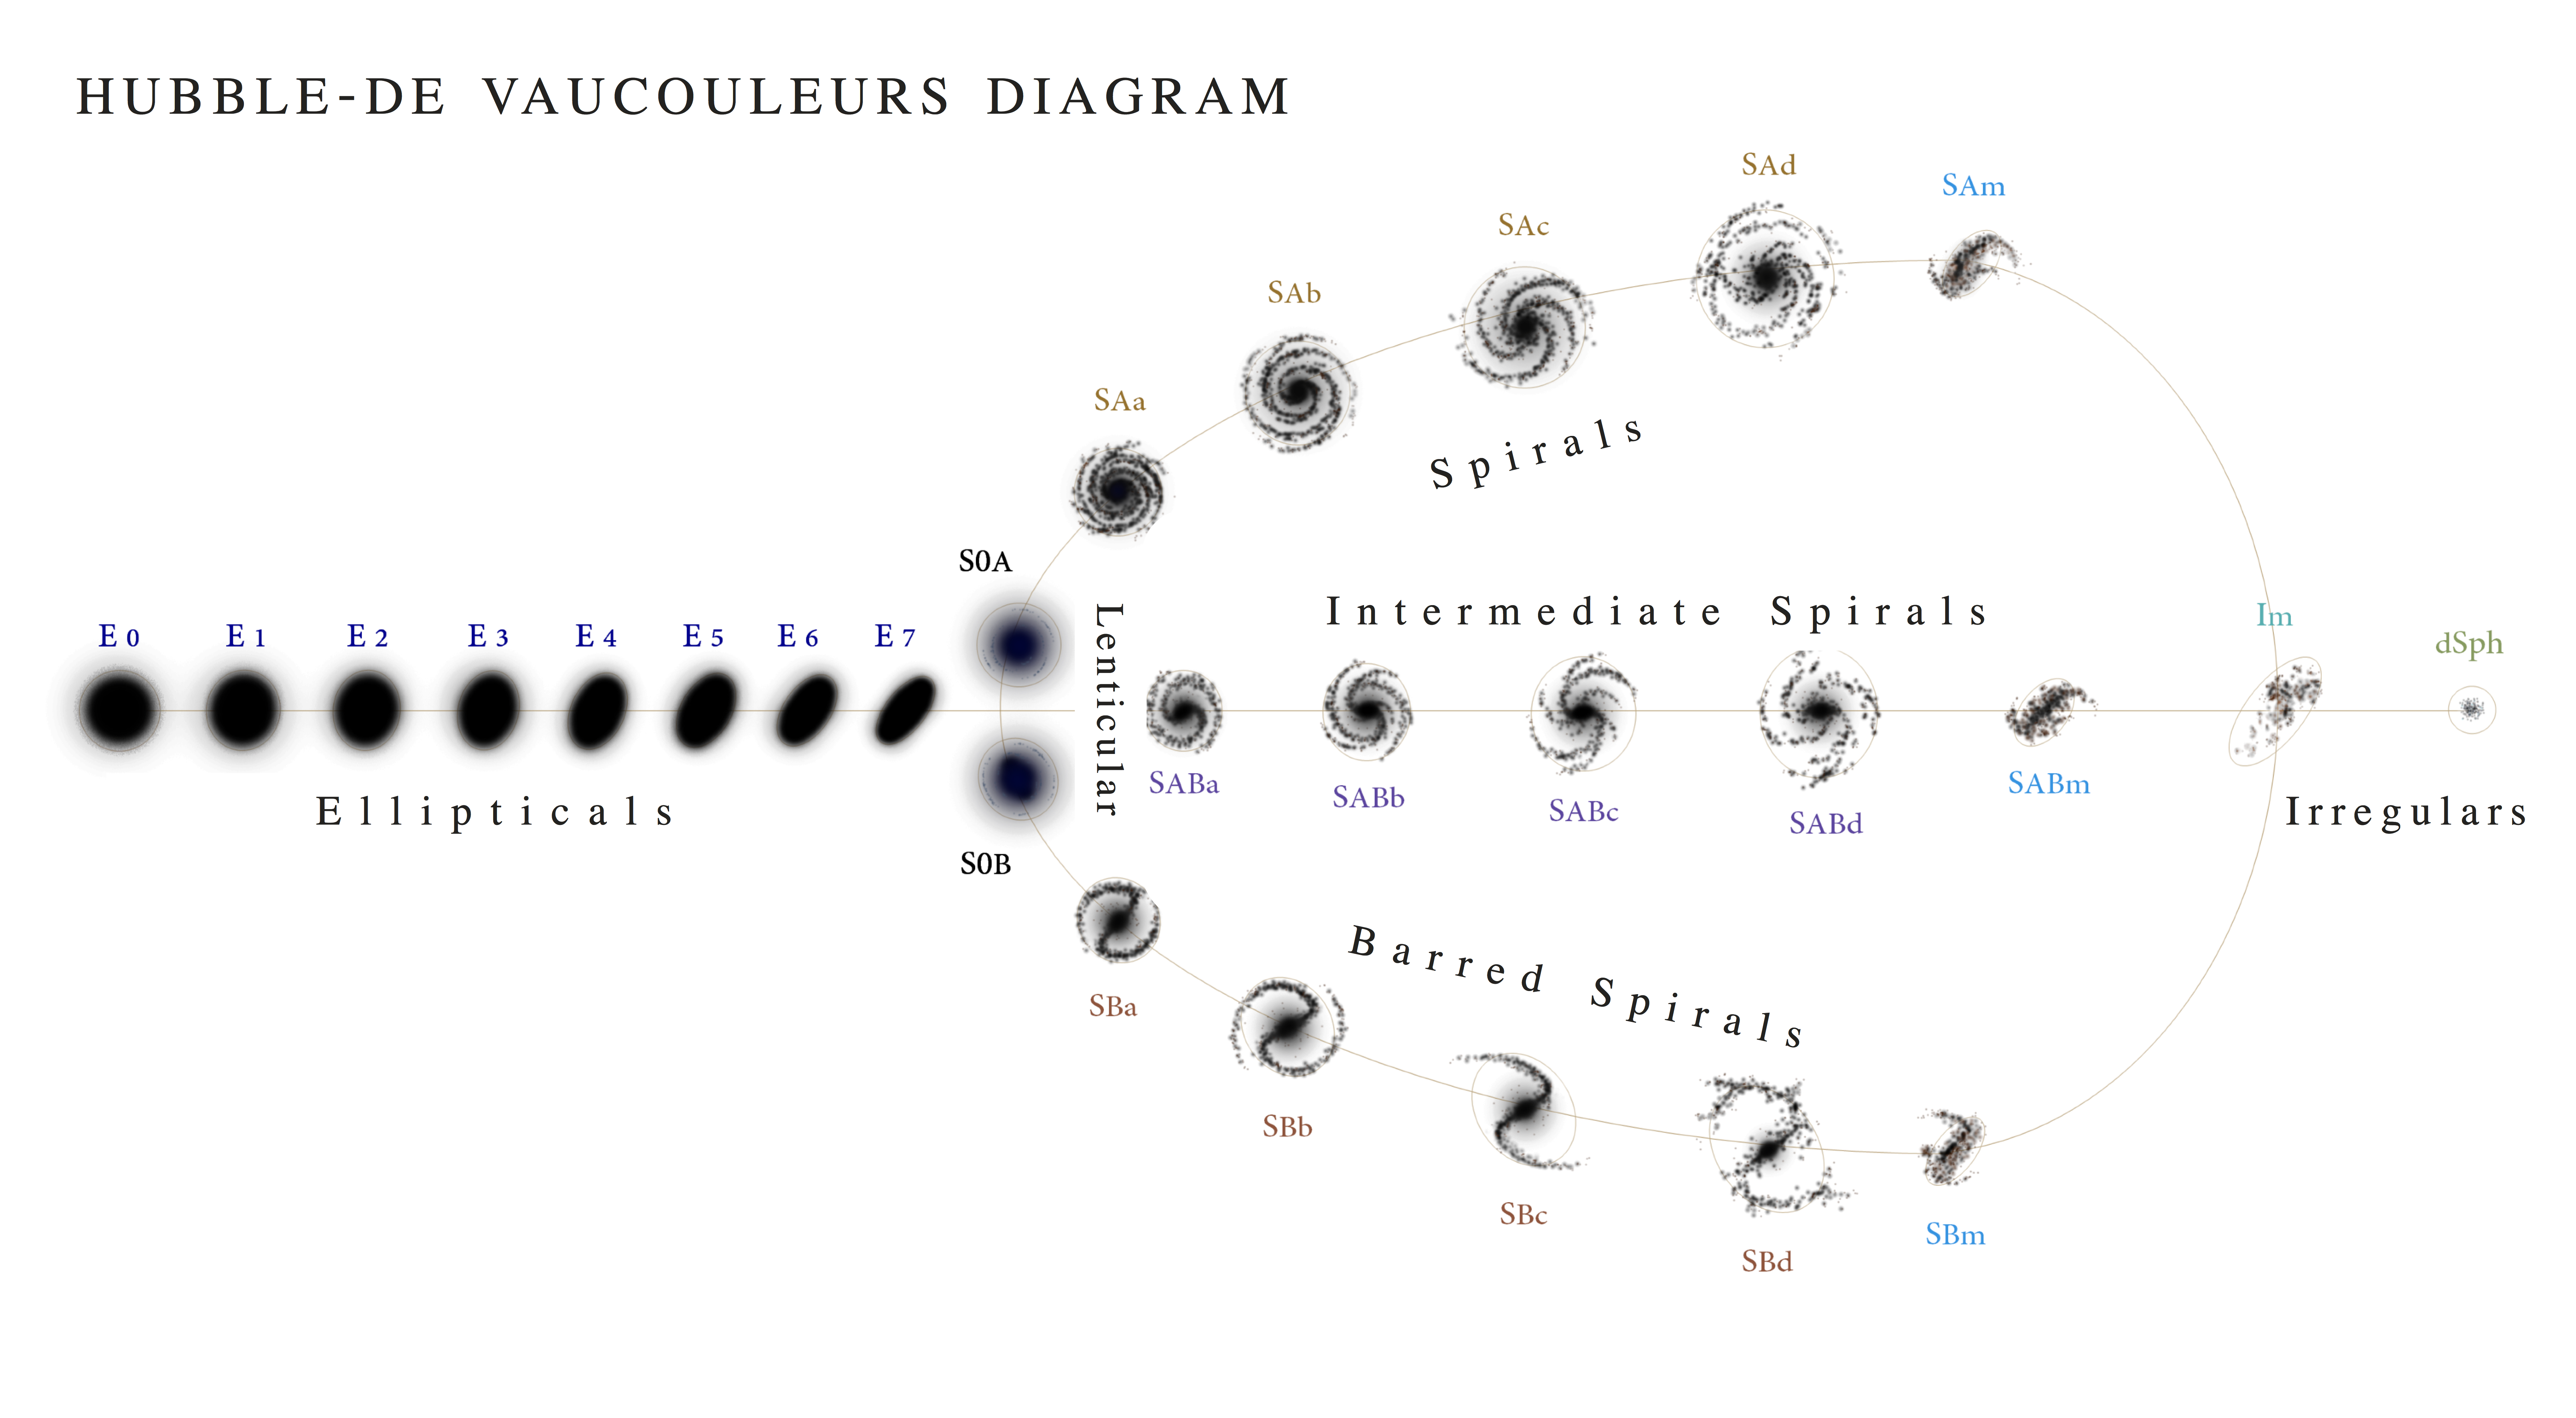
\includegraphics[width=\linewidth]{GalaxyClassificationChart}
	\caption{Hubble-de Vaucouleurs diagram for galaxy morphology.}
	\label{fig:classDiagram}
\end{figure}

Since their discovery, many various types of galaxies have been discovered and categorized into three groups (Figure \ref{fig:classDiagram}\footnote{https://commons.wikimedia.org/wiki/File:Hubble\_-\_de\_Vaucouleurs\_Galaxy\_Morphology\_Diagram.png}).

\subsection{\sc Elliptical Galaxies} \label{ellipticalGalaxies}

\cite{sag} Describes elliptical galaxies as round or elliptical with no visible gas and dust and lacking hot bright stars. These galaxies classified from E0 to E7 based on how elliptical they are.

\subsection{\sc Spiral Galaxies} \label{spiralGalaxies}

Spiral galaxies are the most popular of the classifications of galaxies, and also the most pleasing to the eye. They consist of a disk and spiral arms extruding from their center. Spiral galaxies have some extremely unique characteristics, the least of which are their spiral arms from which they derive their name. A sub-class of spiral galaxy known as the \textit{Barred Spiral Galaxy} is called so because of the presence of a uniquely inherited bar at their center from which their spiral arms protrude.

\subsection{\sc Irregular Galaxies} \label{irregularGalaxies}

Not quite belonging to either the spiral nor the elliptical classes of galaxies, \textit{Irregular Galaxies} are collections of gas and dust with no real structure or shape. An example of irregular galaxies in our own relative backyard would be the Magellanic Clouds. The Small and Large Magellanic Clouds have virtually no proper geometric structure and are interacting gravitationally with our own Milky Way.

\section{\sc Active Galaxies} \label{activeGalaxies}

Thanks to advances in technology, such as the radio and X-Ray telescopes, modern astronomers and physicists have identified a new type of galaxy, the \textit{Active Galaxy}. Active galaxies are galaxies who are theorized to have an actively accreting supermassive black hole at their center. This accretion by the central black hole generates immense amounts of energy across the electromagnetic spectrum. This central black hole and its accompanying accretion disc are known as the nucleus of an active galaxy and are referred to as Active Galactic Nuclei(AGN).

\begin{figure}
	\centering
	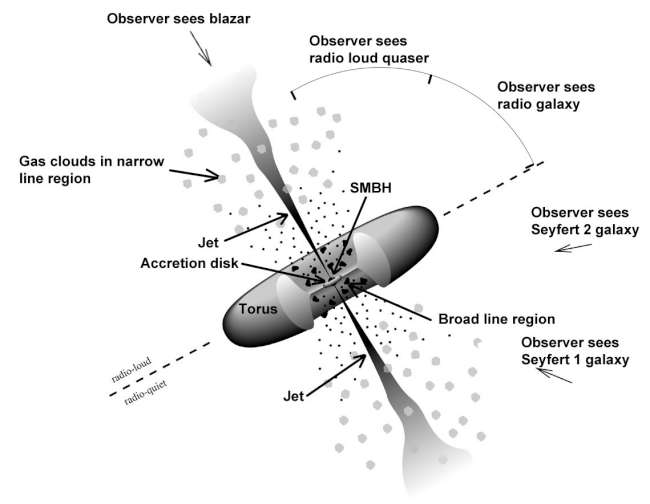
\includegraphics[width=0.6\linewidth]{UnifiedModel}
	\caption{Unified model of Active Galactic Nuclei(AGN).}
	\label{fig:unifiedModel}
\end{figure}

\subsection{\sc The Unified Model} \label{unifiedModel}

In order to help understand what we observe and to help produce new methods of observing AGN, the unified model was developed (Figure \ref{fig:unifiedModel}\footnote{https://fermi.gsfc.nasa.gov/science/eteu/agn/figure1.jpg}). 

In the unified model the nucleus of the active galaxy consists of a supermassive black hole surrounded by a torus of dust and gas from which it is accreting through an accretion disc formed by the gravitational pull of the supermassive black hole. Since there are a number of different types of active galaxies that have been observed, in the unified model this is described by and viewing angle to the galaxy that the observer has. For instance if an observer is viewing an active galaxy from close to edge-on, then they will see either a radio galaxy or a Seyfert 2 AGN. If however they are observing from a higher angle, then the observer will see a quasar or a Seyfert 1 depending on whether the object is radio loud or not. And finally observing from an angle equivalent to directly above will result in the observer viewing a blazar.

\section{\sc Black Holes} \label{blackHole}

To understand black holes, one must first understand escape velocity and how it relates to astronomical objects. For any given object, the escape velocity is the velocity required by any object or particle in order for that object or particle to escape the gravitational well created by the initial object. For example, in order for a probe to leave our Earth and visit the other planets of our solar system, that probe must first reach the escape velocity for the Earth. Mathematically speaking the escape velocity is defined as:
\begin{equation} \label{eqn1.1}
v_{e} = \sqrt{\frac{2GM}{r}}
\end{equation}
where $v_{e}$ is the escape velocity, $G$ is the universal gravitational constant, $M$ is the mass of the object to escape from, and $r$ is the distance from the center of said object. When $v_{e} \geq c$ at a given $r$, where $c$ is the speed of light, then nothing, not even light can escape the gravitational well created by the object in question.

In this case the object in question would be referred to as a black hole and the radius from the center of the object $r$ is defined as the event horizon. There exists a more in depth definition for the black hole that will be discussed in section \ref{generalRelativity}. Black holes are commonly classified according to their mass due to the relationship between their mass and the radius of their event horizon, given by:
\begin{equation} \label{eqn1.2}
r_{s} = \frac{2GM}{c^{2}}
\end{equation}
where $r_{s}$ is the Schwarzchild radius as defined in chapter \ref{generalRelativity}.

\subsection{\sc Stellar Mass Black Holes} \label{stellarBH}

Stellar mass black holes are those black holes that are most commonly depicted in fiction and film. With masses ranging from $10\textup{M}_{\odot}$ to $10^{2}\textup{M}_{\odot}$ where $\textup{M}_{\odot}$ is the mass of our Sun, know as a solar mass.

\subsection{\sc Intermediate-Mass Black Holes} \label{intermediateBH}

Intermediate-mass black holes(IMBH) are theorized to to be those black holes with significantly more mass than a stellar mass black hole but less than a supermassive black hole. There have been a couple of IMBH candidates in our own galaxy and others nearby. Intermediate-mass black holes have masses between $10^{2}\textup{M}_{\odot}$ and $10^{5}\textup{M}_{\odot}$ Since this thesis is concerned with AGN and thus supermassive black holes, we will not discuss IMBHs in more detail.

\subsection{\sc Supermassive Black Holes}

With masses ranging from $10^{5}\textup{M}_{\odot}$ and up, supermassive black holes are believed to be at the centers of most large galaxies holding them together. There is observational evidence that our own Milky Way is host to one such monster, Sagittarius A*. When one of these supermassive black holes is actively accreting from its surrounding galaxy, we can it the nuclei of an active galaxy as discussed in section \ref{activeGalaxies}.

\section{\sc How AGN are Observed} \label{howObserved}

Since AGN are so far away and their central engines so massive that light cannot escape them, how then can we observe them? The answer to that question is that we cannot and still have not \textit{directly} observed one yet. We can however indirectly observe them, by their gravitational effect on their surroundings, and in the case of AGN by observing the emission they produce through their accretion process.

As discussed earlier in section \ref{activeGalaxies}, the supermassive black holes at their centers are undergoing active accretion. This process drags matter in toward the black hole in a spiral at increasing speeds. The matter around the black hole spins as it approaches because it must conserve angular momentum. As such, the gas and dust in the area around the nucleus of an AGN forms a torus, which then thins into a disc as it approaches the event horizon. As matter from the torus gets closer to the event horizon, its velocity increases, heating it up to temperatures such that it eventually becomes ionized at the innermost stable circular orbit(ISCO).

On the accretion disc matter becomes hot enough to emit light in the Ultra-Violet(UV) range, and electrons are striped and deposited into clouds above and below the disc. In these electron clouds, UV light rays collide with electrons and sap energy from them in a process know as Reverse Compton Scattering, commonly referred to as Comptonisation. The UV rays that undergo this Comptonising process are re-emitted at high energies, often in the X-Ray band but also up to and including the gamma ray band.

\subsection{\sc Light-Curves} \label{lightcurves}
Thanks to the processes in and around the accretion disc, AGN emit light almost evenly across the entire electromagnetic spectrum. This allows us to collect the light they emit in our direction using telescopes and computer processes to generate what are known as light-curves. Light-curves are a comparison of $erg/s$ to the wavelength, frequency, or energy level of light particles. In SI units, $erg/s$ is equivalent to $\frac{\textup{W}\cdot kg\cdot m^{2}}{s^{3}}$. When observing AGN it is common to refer to wavelengths of light by their corresponding energy levels in $keV$. Since light behaves in expected ways when interacting in different environments, elemental spectral lines for example, modern astronomers use the light-curves of AGN to gain insight into their inner workings.

Some expected properties of the spectra obtained from AGN are, the presence of an iron line around the $6.5 keV$ mark, a falloff in photon counts as photon energy increases, and obscuring of the lower energy X-ray and higher energy UV range due to absorption in the torus and surrounding gas and dust around the central engine.

\newpage

\subsection{\sc Orbital X-Ray telescopes} \label{xrayTelesopes}

\begin{figure}
	\centering
	\begin{minipage}{0.45\textwidth}
		\centering
		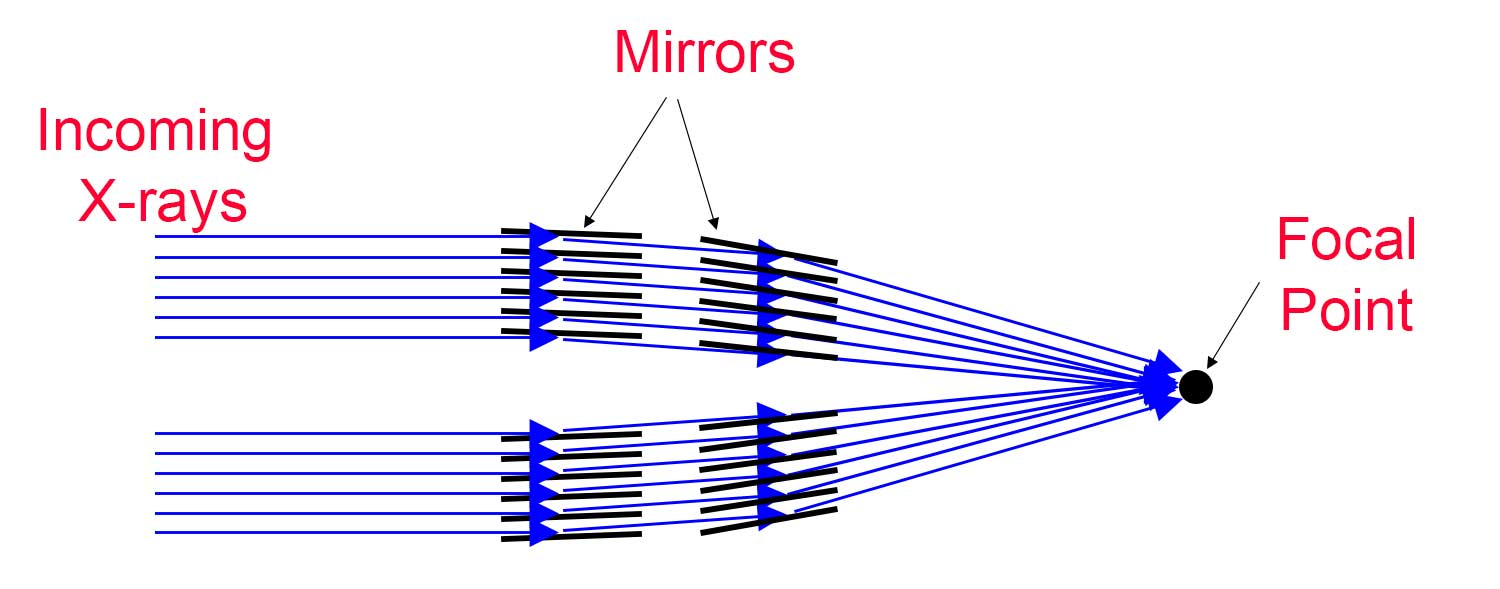
\includegraphics[width=\linewidth]{xrayTelescopeMultimirror}
		\caption{X-Ray telescope cutaway diagram.}
		\label{fig:xrayMultiMirror}
	\end{minipage}
	\begin{minipage}{0.45\textwidth}
		\centering
		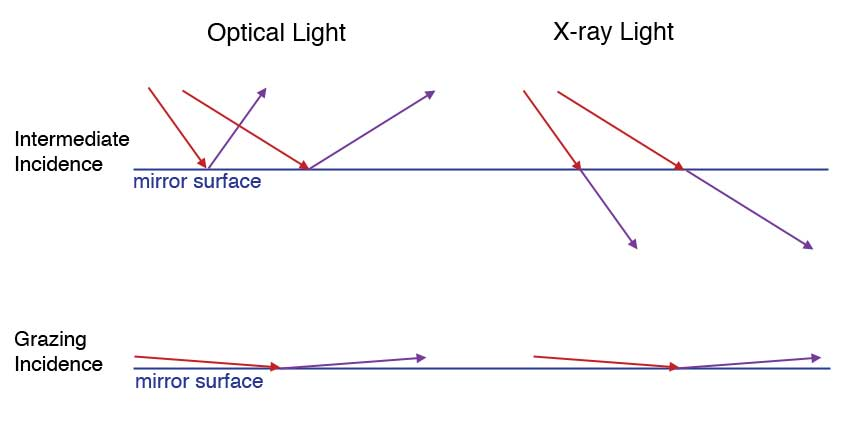
\includegraphics[width=\linewidth]{grazingIncidence}
		\caption{Grazing incidence diagram.}
		\label{fig:grazingIncidence}
	\end{minipage}
\end{figure}

As discussed in the previous section \ref{lightcurves}, AGN produce light almost evenly across the electromagnetic spectrum. The section that astronomers and physicists studying AGN find the most interesting is the UV to X-Ray region. In order to observer AGN without the distortions produced by our atmosphere and other terrestrial effects, orbital satellite telescopes are used. For this project the Neil Gehrels \textit{Swift} Observatory was used. The \textit{Swift} orbital telescope is equipped with a UV/Optical telescope, capable of obtaining spectra in the UV and optical, what we can see, wavebands. \textit{Swift} is also equipped with an X-Ray telescope for obtaining spectra in the X-ray band of the EM spectrum. The X-Ray telescope uses many mirrors at slightly increasing angles positioned throughout to focus the incoming X-rays as shown in (Figure \ref{fig:xrayMultiMirror}\footnote{https://imagine.gsfc.nasa.gov/observatories/technology/xray\_telescopes1.html \label{xrayTelescopeRef}}). The mirrors must be placed at slightly increasing angles because otherwise, the high energy X-Rays would pass right through the mirrors, unlike optical light (Figure \ref{fig:grazingIncidence}\textsuperscript{\ref{xrayTelescopeRef}}).

\section{\sc Project Goals} \label{expectedAchievements}

This project focused on analyzing the light-curves of several AGN using a Structure Function. The Structure Function, as will be discussed in section \ref{structureFunction}, is similar to a Fourier Analysis but without the aliasing and windowing issues that arise from unevenly sampled data. Since many astronomical objects cannot produce evenly sampled data due to the methods of observation and the timescales on which astronomical events happen, this project aims to provide a method for observing and analyzing astronomical events and objects such as AGN through the use of a Structure Function to help identify time-scales on which significant events might be occurring.

\chapter{\sc General Relativistic Description of Black Holes} \label{generalRelativity}

A brief description of general relativity, its origins, and why it relates to this project.

\section{\sc An introduction to Tensors} \label{tensorIntro}

An introduction to tensors and their mathematical properties

\section{\sc The Metric Tensor} \label{metricTensor}

Role of the metric tensor

\section{\sc The Spacetime Interval} \label{spacetimeInterval}

Role of the spacetime interval

\section{\sc Black Hole Solutions} \label{blackHoleSolutions}

Overview of black hole solutions

\subsection{\sc The Schwarzchild Solution} \label{schwarzchildSolution}

The mathematics of the Schwarzchild solution.

\subsection{\sc The Kerr Solution} \label{kerrSolution}

The mathematics of the Kerr solution.

\subsection{\sc Properties of the Kerr Solution} \label{kerrSolutionProperties}

Properties of the Kerr solution.

\chapter{\sc Statistical Analysis} \label{statisticalAnalysis}

Data collected on AGN is often difficult to work with, as mentioned in section \ref{activeGalaxies}, it is often unevenly sampled posing challenges to astronomers and physicists. Unevenly sampled data often causes aliasing and windowing when analyzed using conventional methods such as a Fourier-based power spectrum analysis. For this reason the method of structure function analysis was chosen, as it partially minimizes both aliasing and windowing. The structure function also has the added advantage of remaining in the time domain as opposed to the frequency domain as does the Fourier-based analysis. For these reasons the structure function was the method of choice for the analysis conducted in this project.

\section{\sc The Structure Function} \label{structureFunction}

The structure function is discussed by \citep{cordes1985} in their appendix and was originally defined by \citep{rutman}. It can be closely compared to the auto-correlation and cross-correlation functions. Structure functions of order $M$ remove polynomials of order $M-1$ from the time series leaving a result that is dependent only on on any stationary random process inherent in the time series and any higher order polynomial trends.

\subsection{\sc Definition of the Structure Function} \label{structureFunctionDefinition}

For any given random process the $M^{th}$ order structure function is defined by \cite{rutman} as:
\begin{equation} \label{eqn3.1}
D^{\left(M\right)}_{\phi}\left(t, \tau\right) = \langle\left[\Delta^{\left(M\right)}_{\phi}\left(t, \tau\right)\right]^{2}\rangle
\end{equation}
where the angled brackets are an average over time $t$. \cite{rutman} also defines the $M^{th}$ increment of $\phi\left(t\right)$ as:
\begin{equation} \label{eqn3.2}
\Delta^{\left(M\right)}_{\phi}\left(t, \tau\right) = \sum_{n=0}^{\infty}\left(-1\right)^{n}{M \choose n}\phi\left(t + \left[M - n\right]\tau\right)
\end{equation}

For a time series of measurements $f\left(t_{i}\right), i = 1,2,3,...$ the first order structure is defined by \citep{collier2001} as:
\begin{equation}
S\left(\tau\right) = \frac{1}{N\left(\tau\right)}\sum_{i<j}\left[f\left(t_{i}\right)-f\left(t_{j}\right)\right]^{2}
\end{equation}
where the sum is over all pairs $\left(f\left(t_{i}\right),f\left(t_{j}\right)\right)$ for which $t_{j}-t_{i}=\tau$, and $N\left(\tau\right)$ is the number of such pairs.

\subsection{\sc Shape and Characteristics} \label{shapeAndCharacteristics}

\begin{figure}
	\centering
	\begin{minipage}{0.45\textwidth}
		\centering
		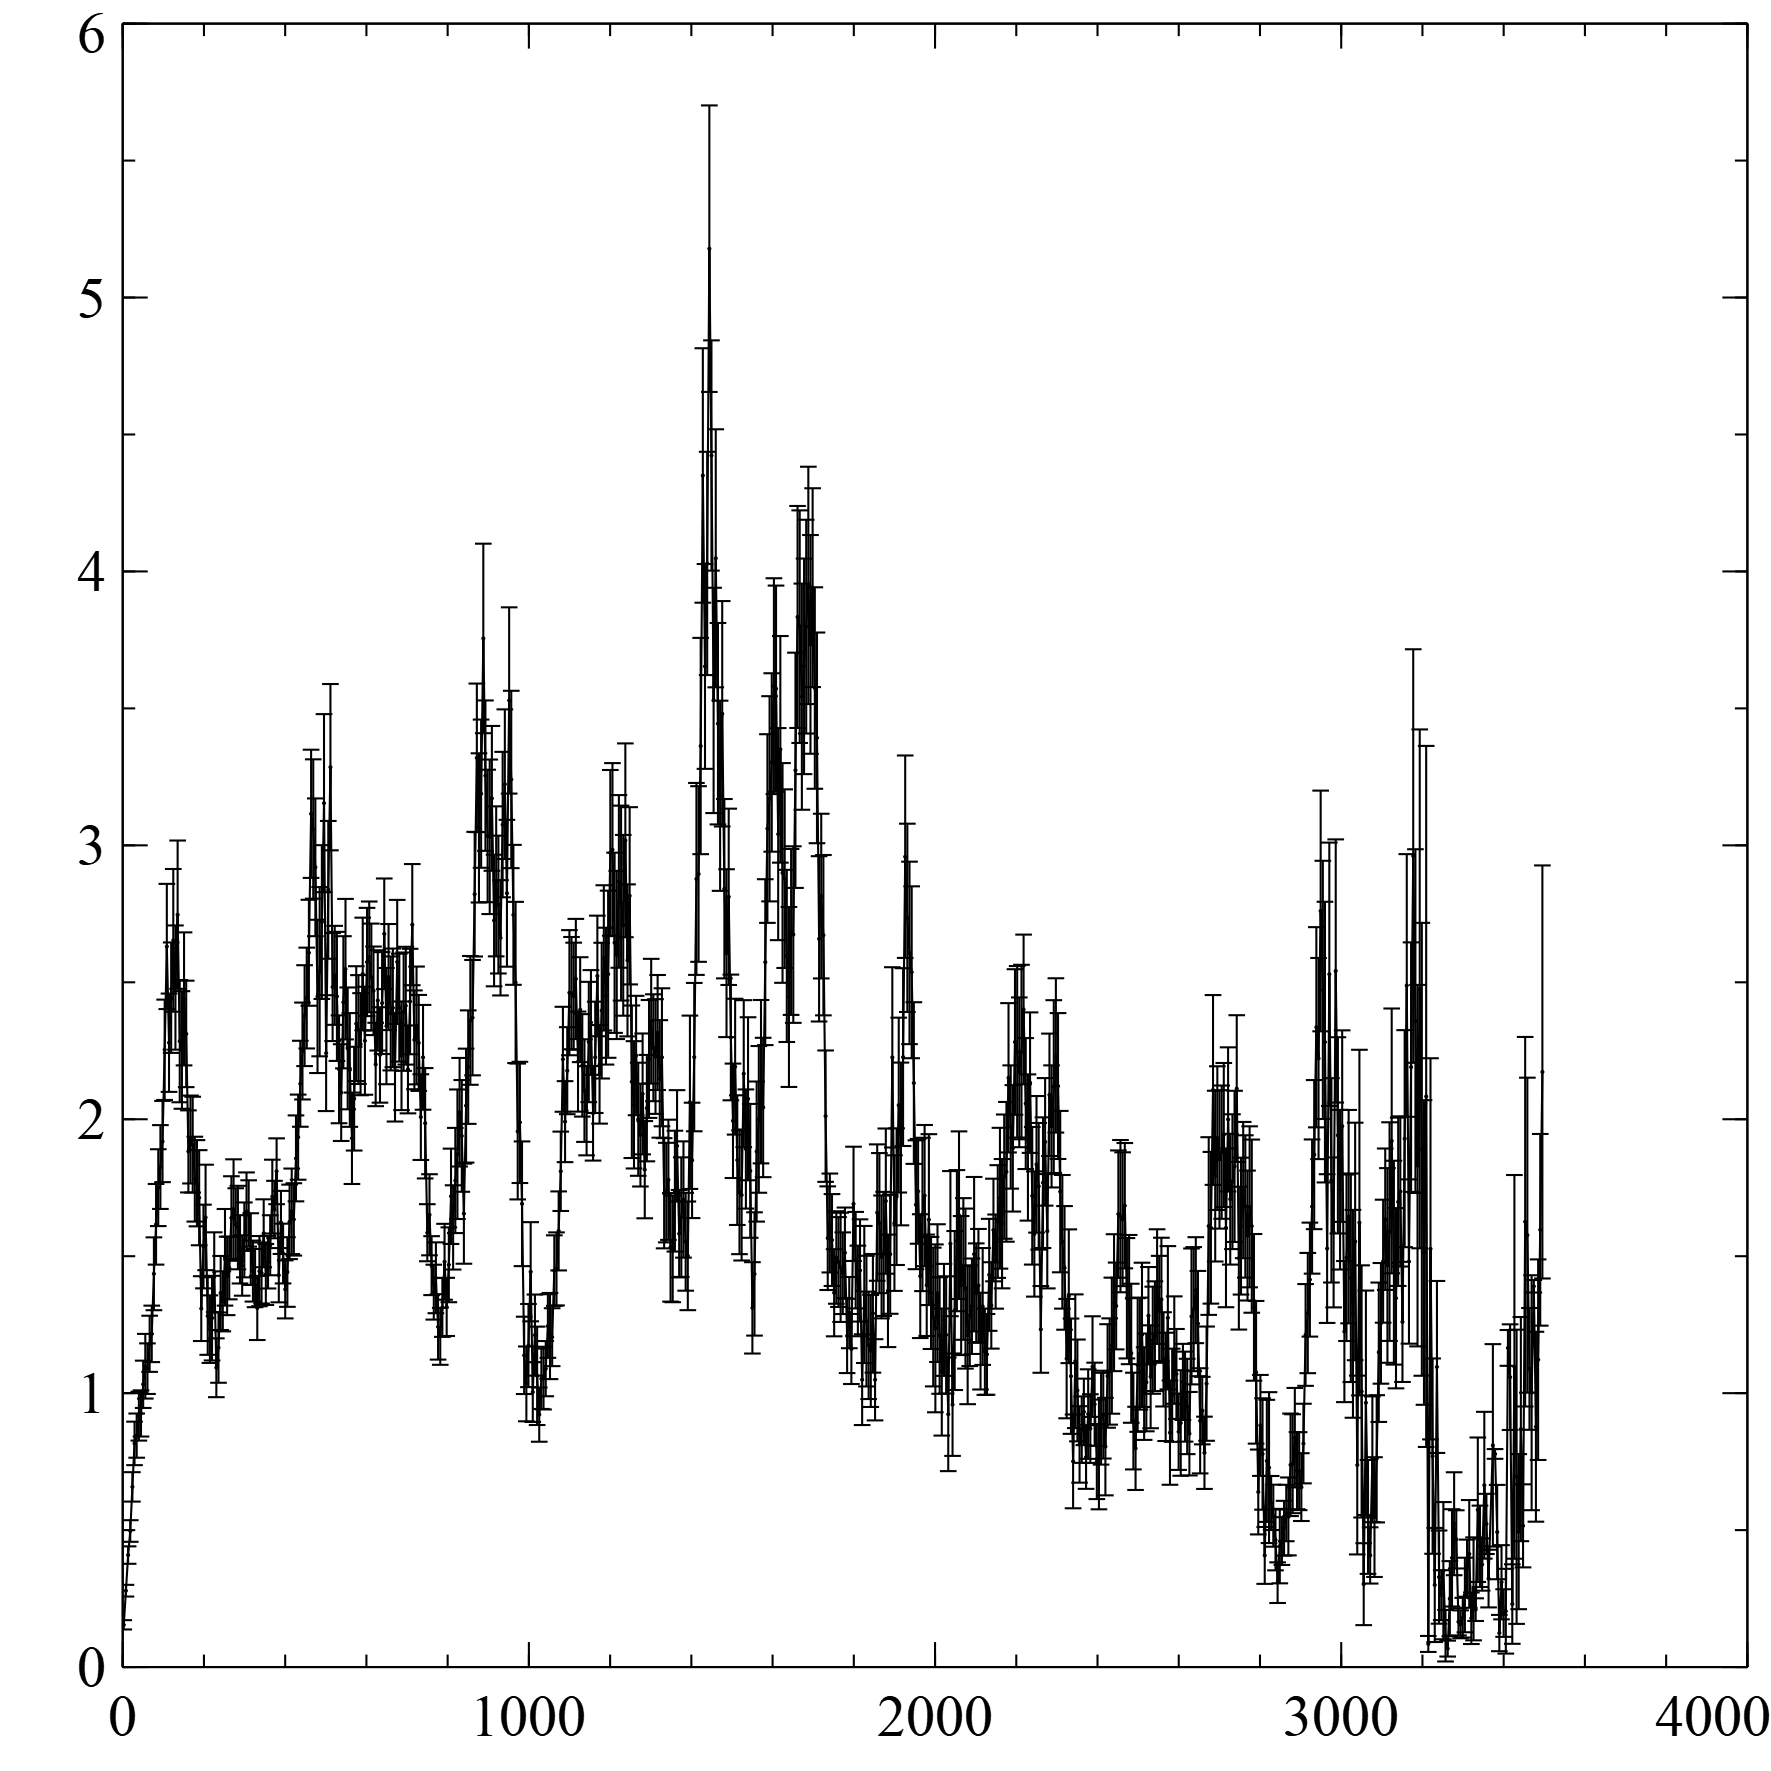
\includegraphics[width=0.8\linewidth]{structureFunctionShape}
		\caption{An example of a structure function with normal scaled axes.(To be replaced)}
		\label{fig:structureFunctionShape}
	\end{minipage}
	\begin{minipage}{0.1\textwidth}
	\end{minipage}
	\begin{minipage}{0.45\textwidth}
		\centering
		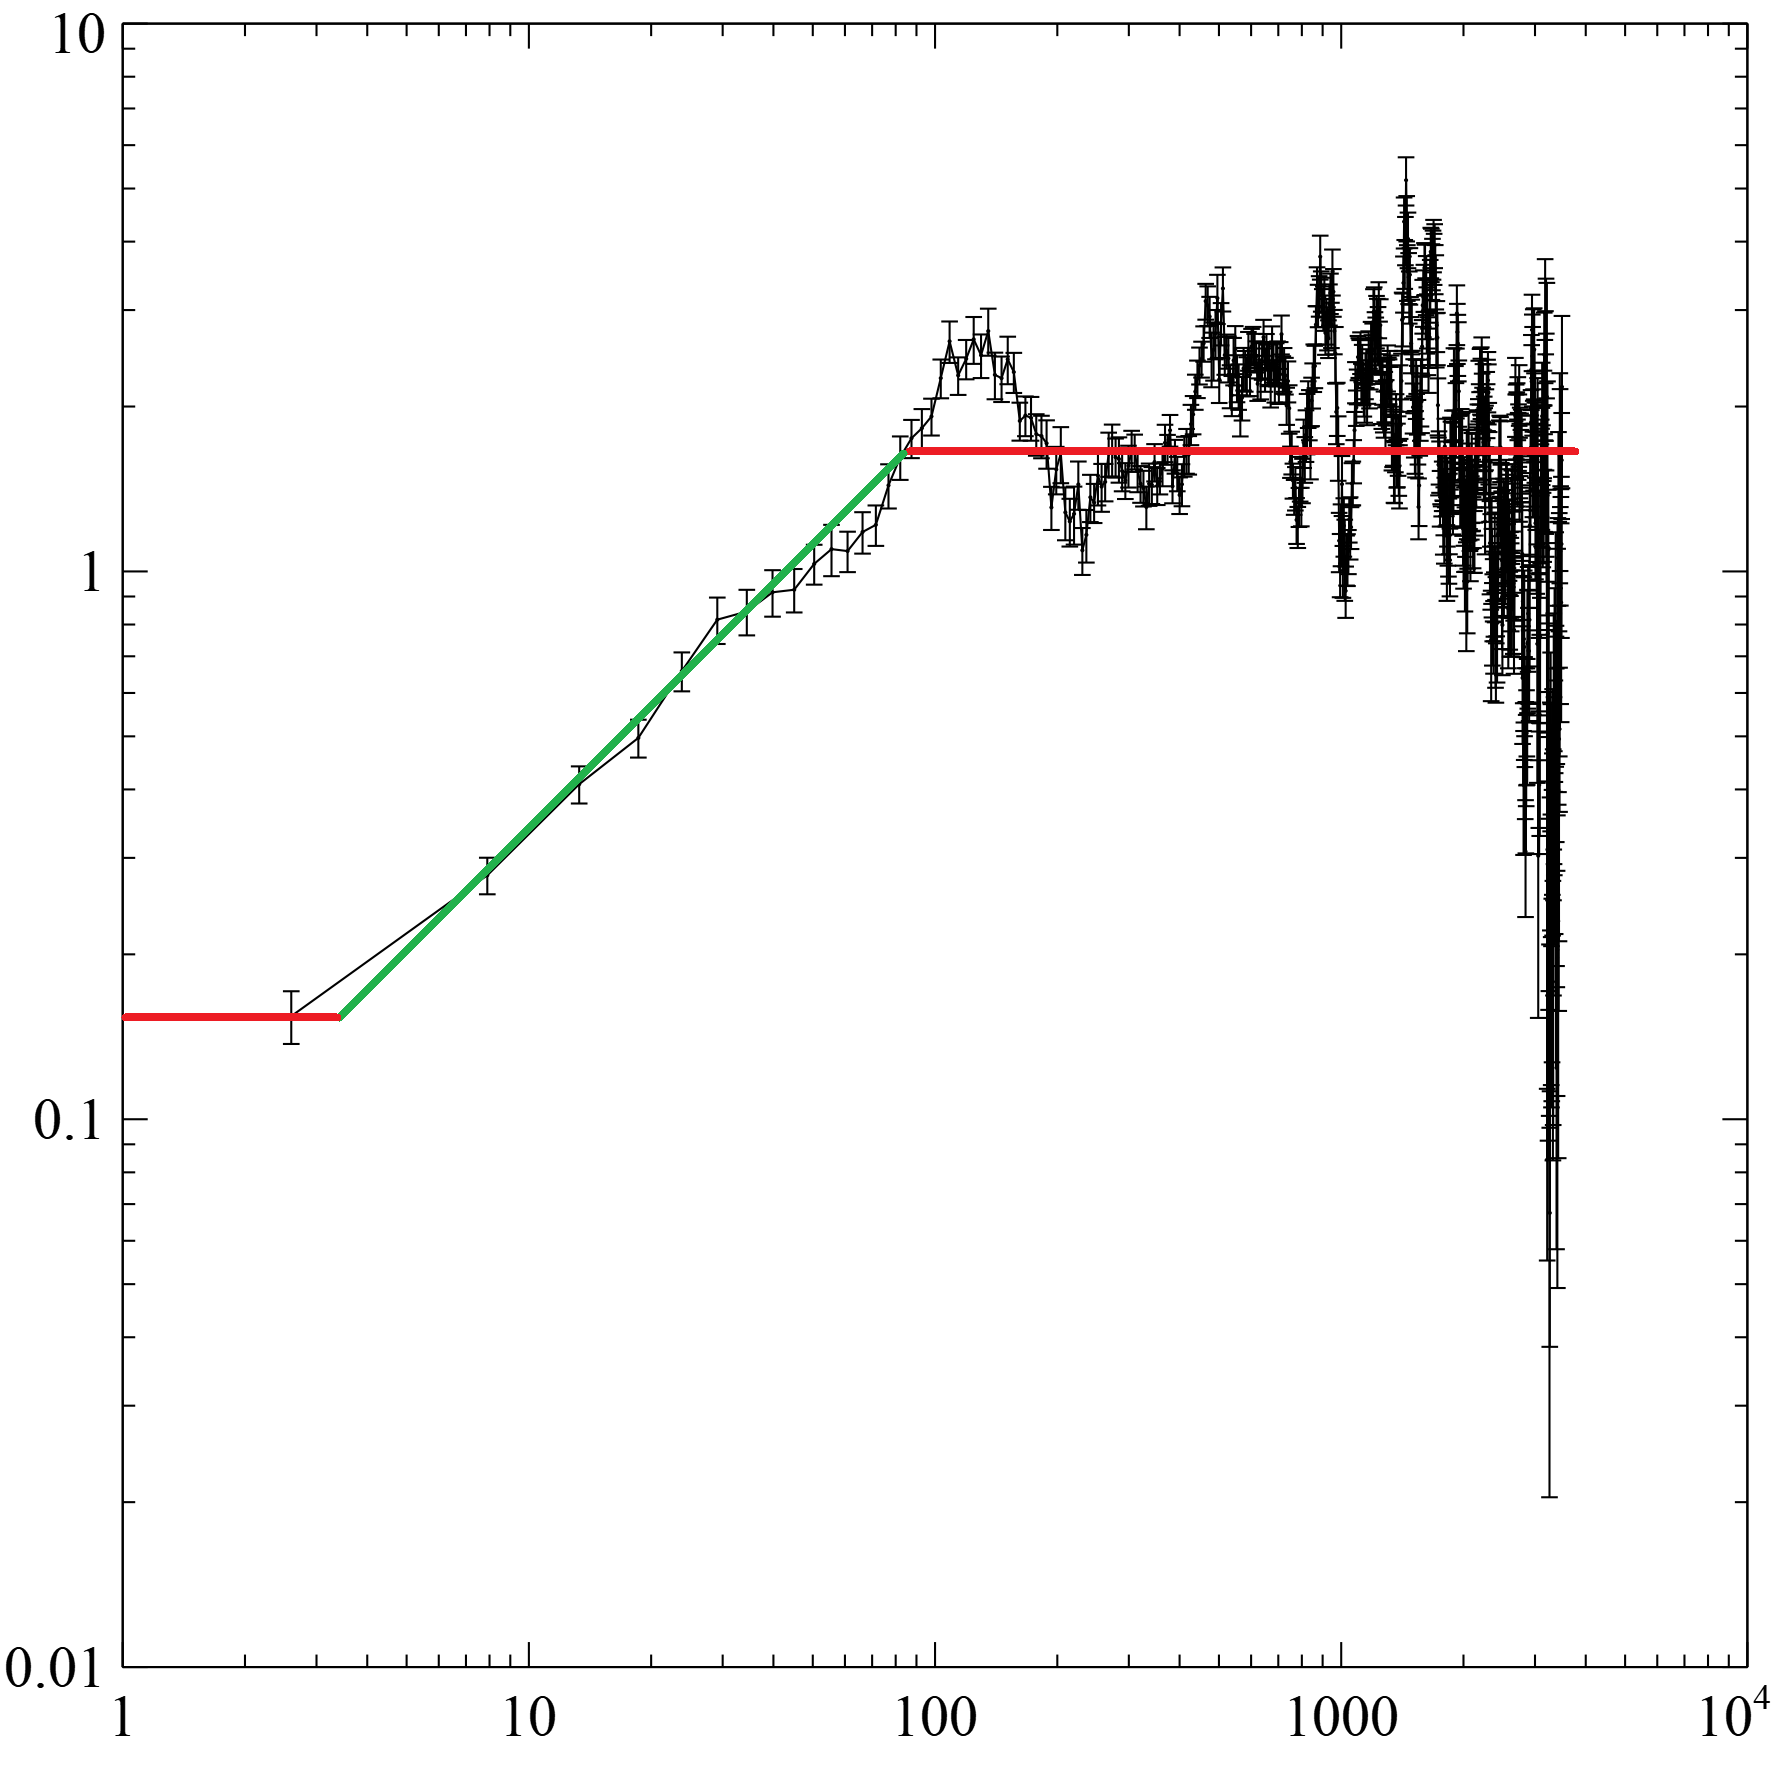
\includegraphics[width=0.8\linewidth]{structureFunctionLogShape}
		\caption{An example of a structure function with log scaled axes. (To be replaced)}
		\label{fig:structureFunctionLogShape}
	\end{minipage}
\end{figure}

Structure functions have a very distinct shape, resembling a sigmoid but dominated by twice the signal variance, $2\sigma^{2}$, on short timescales and twice the noise variance, $2\sigma_{noise}^{2}$, on long timescales. This results in two noise dominated plateaus connected by a power-law section as shown in figure \ref{fig:structureFunctionLogShape} where the plateaus are shown with a red line and the power-law section is shown with a green line overlaid on top of real data for a structure function. As is evident in figure \ref{fig:structureFunctionLogShape}, the upper plateau, corresponding to longer timescales, is completely noise dominated.

The power-law region of the structure function exists where $\tau_{min}\lesssim\tau\lesssim\tau_{max}$. When $\tau_{max}\ll T$, where $T$ is the total duration of the time-series, we can approximate $\tau_{max}$ to a characteristic timescale, $\tau_{char}$, determined by fundamental source characteristics such as mass, size, matter propagation and others depending on the source of the time-series.

\subsection{\sc Problems and Pitfalls} \label{problemsAndPitfalls}

\begin{figure}
	\centering
	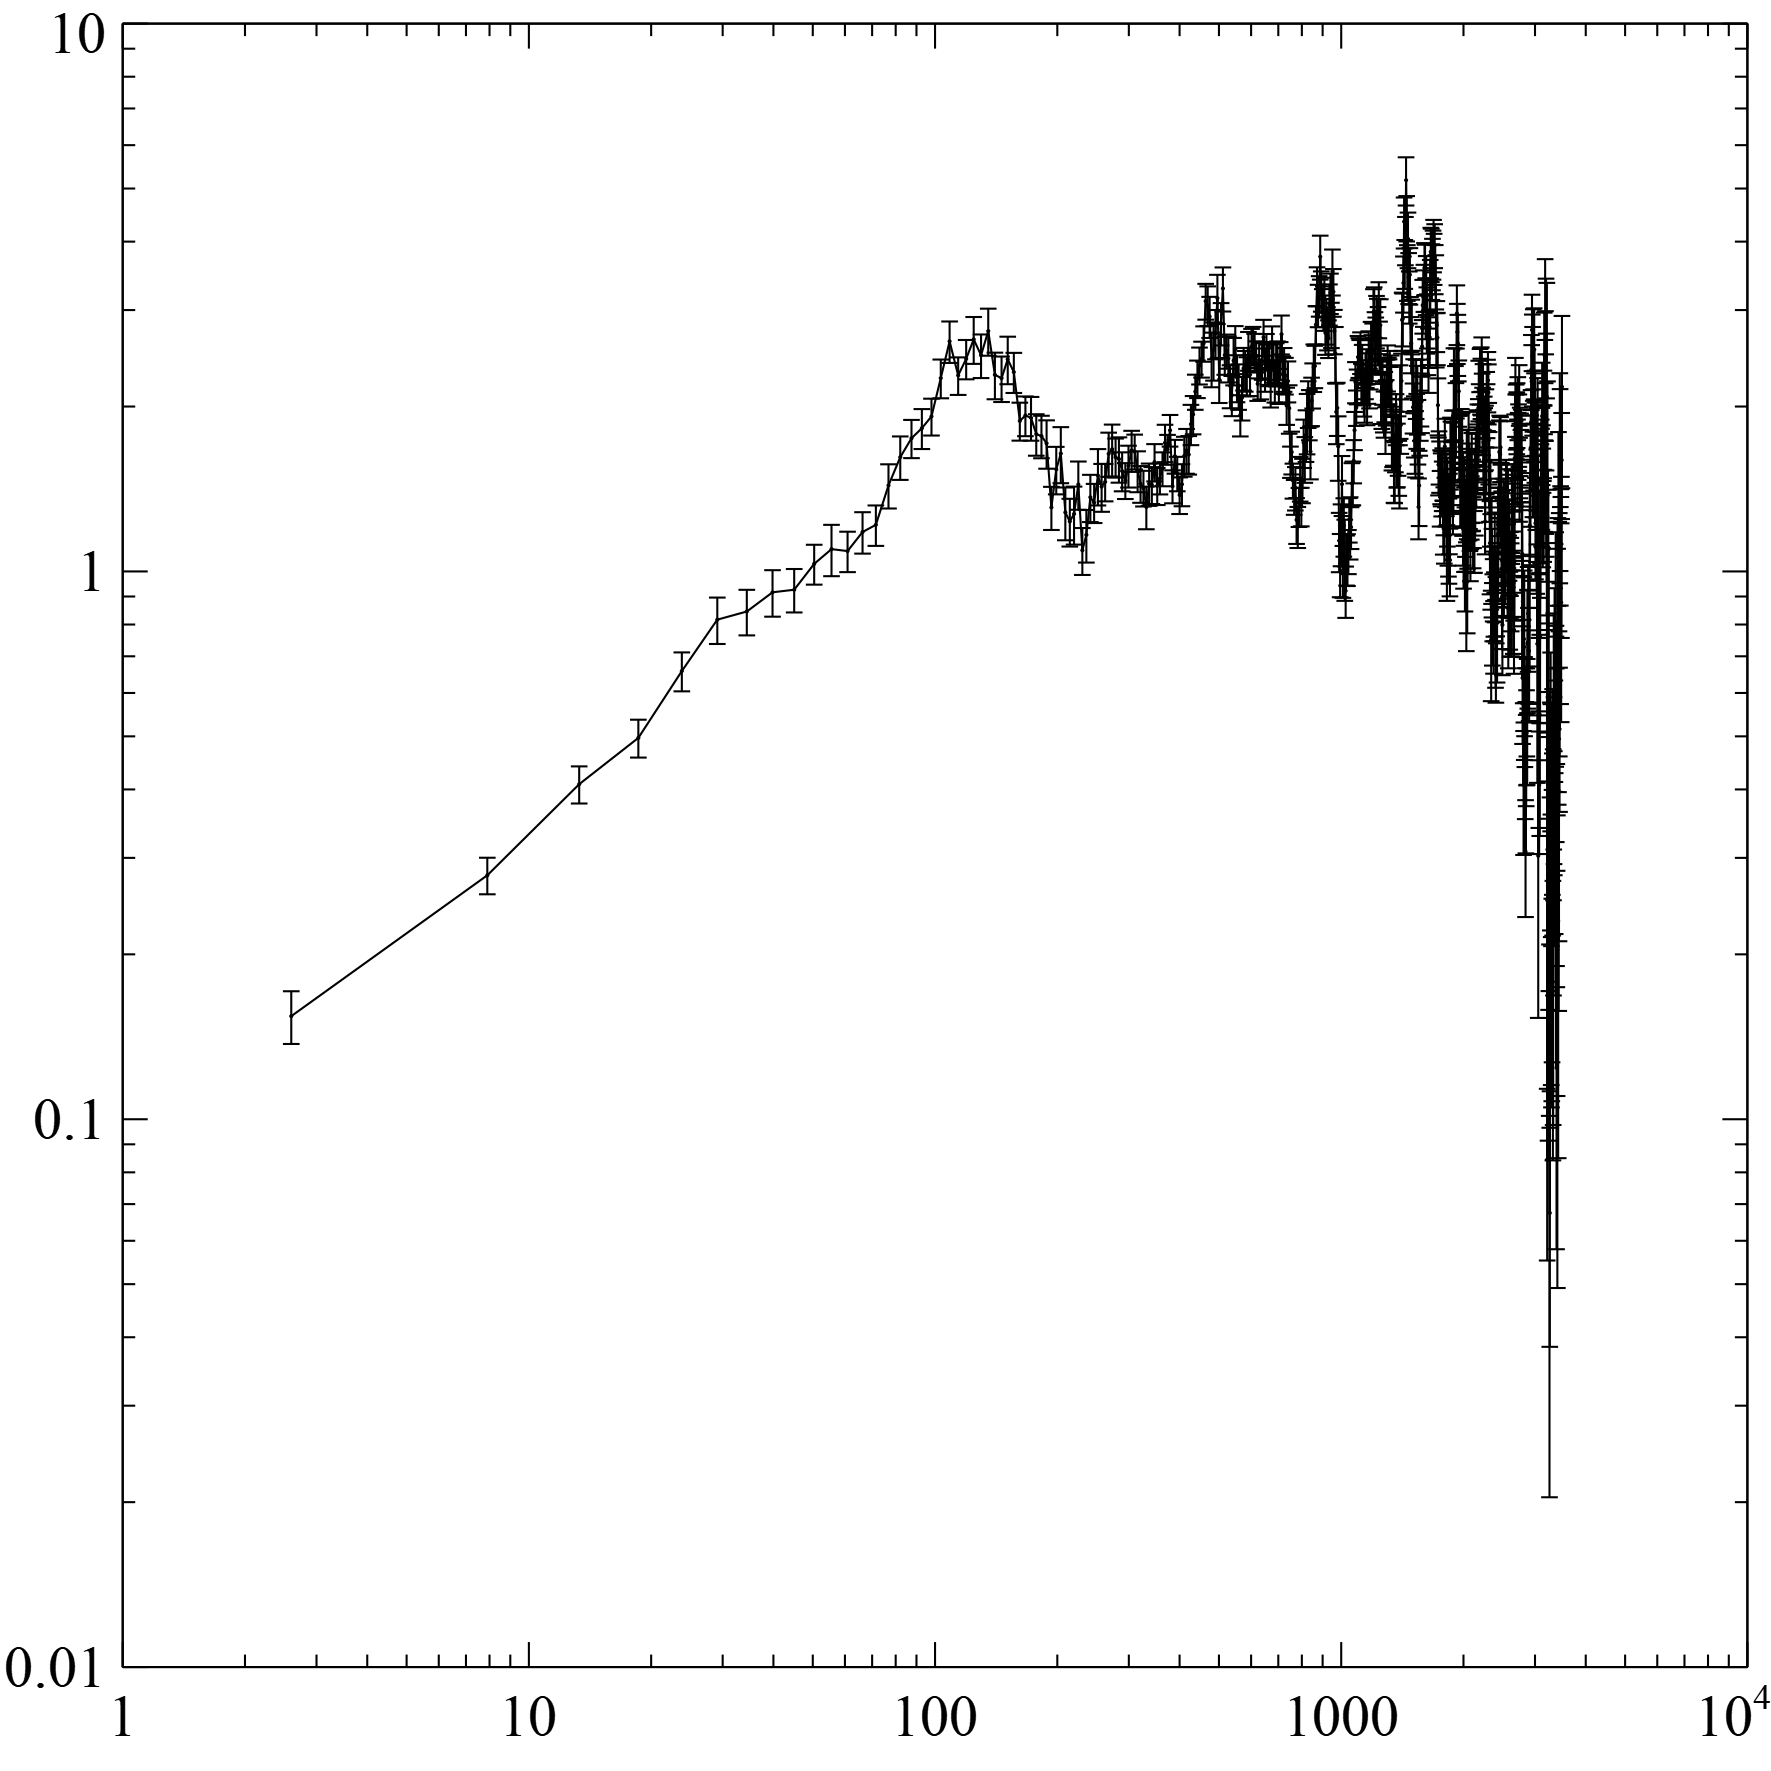
\includegraphics[width=0.4\linewidth]{mkn335UVW2SF}
	\caption{Structure function for UVW2 data collected from Mkn335}
	\label{fig:mkn335UVW2SF}
\end{figure}

The structure functions is an extremely valuable tool for analyzing data that has odd or uneven sampling rates, but it is not without fault. Some things to be aware of when using a structure function on data are as follows. Linear trends that span the entire time-series will artificially steepen the structure function. This can be avoided by removing a best-fit linear model applied to the entire time-series. Some object may have more than one characteristic timescale and this may manifest itself as a third plateau breaking the power-law region in two, as can be seen in figure \ref{fig:mkn335UVW2SF}. 

\section{\sc The Data} \label{theData}

\begin{figure}
	\centering
	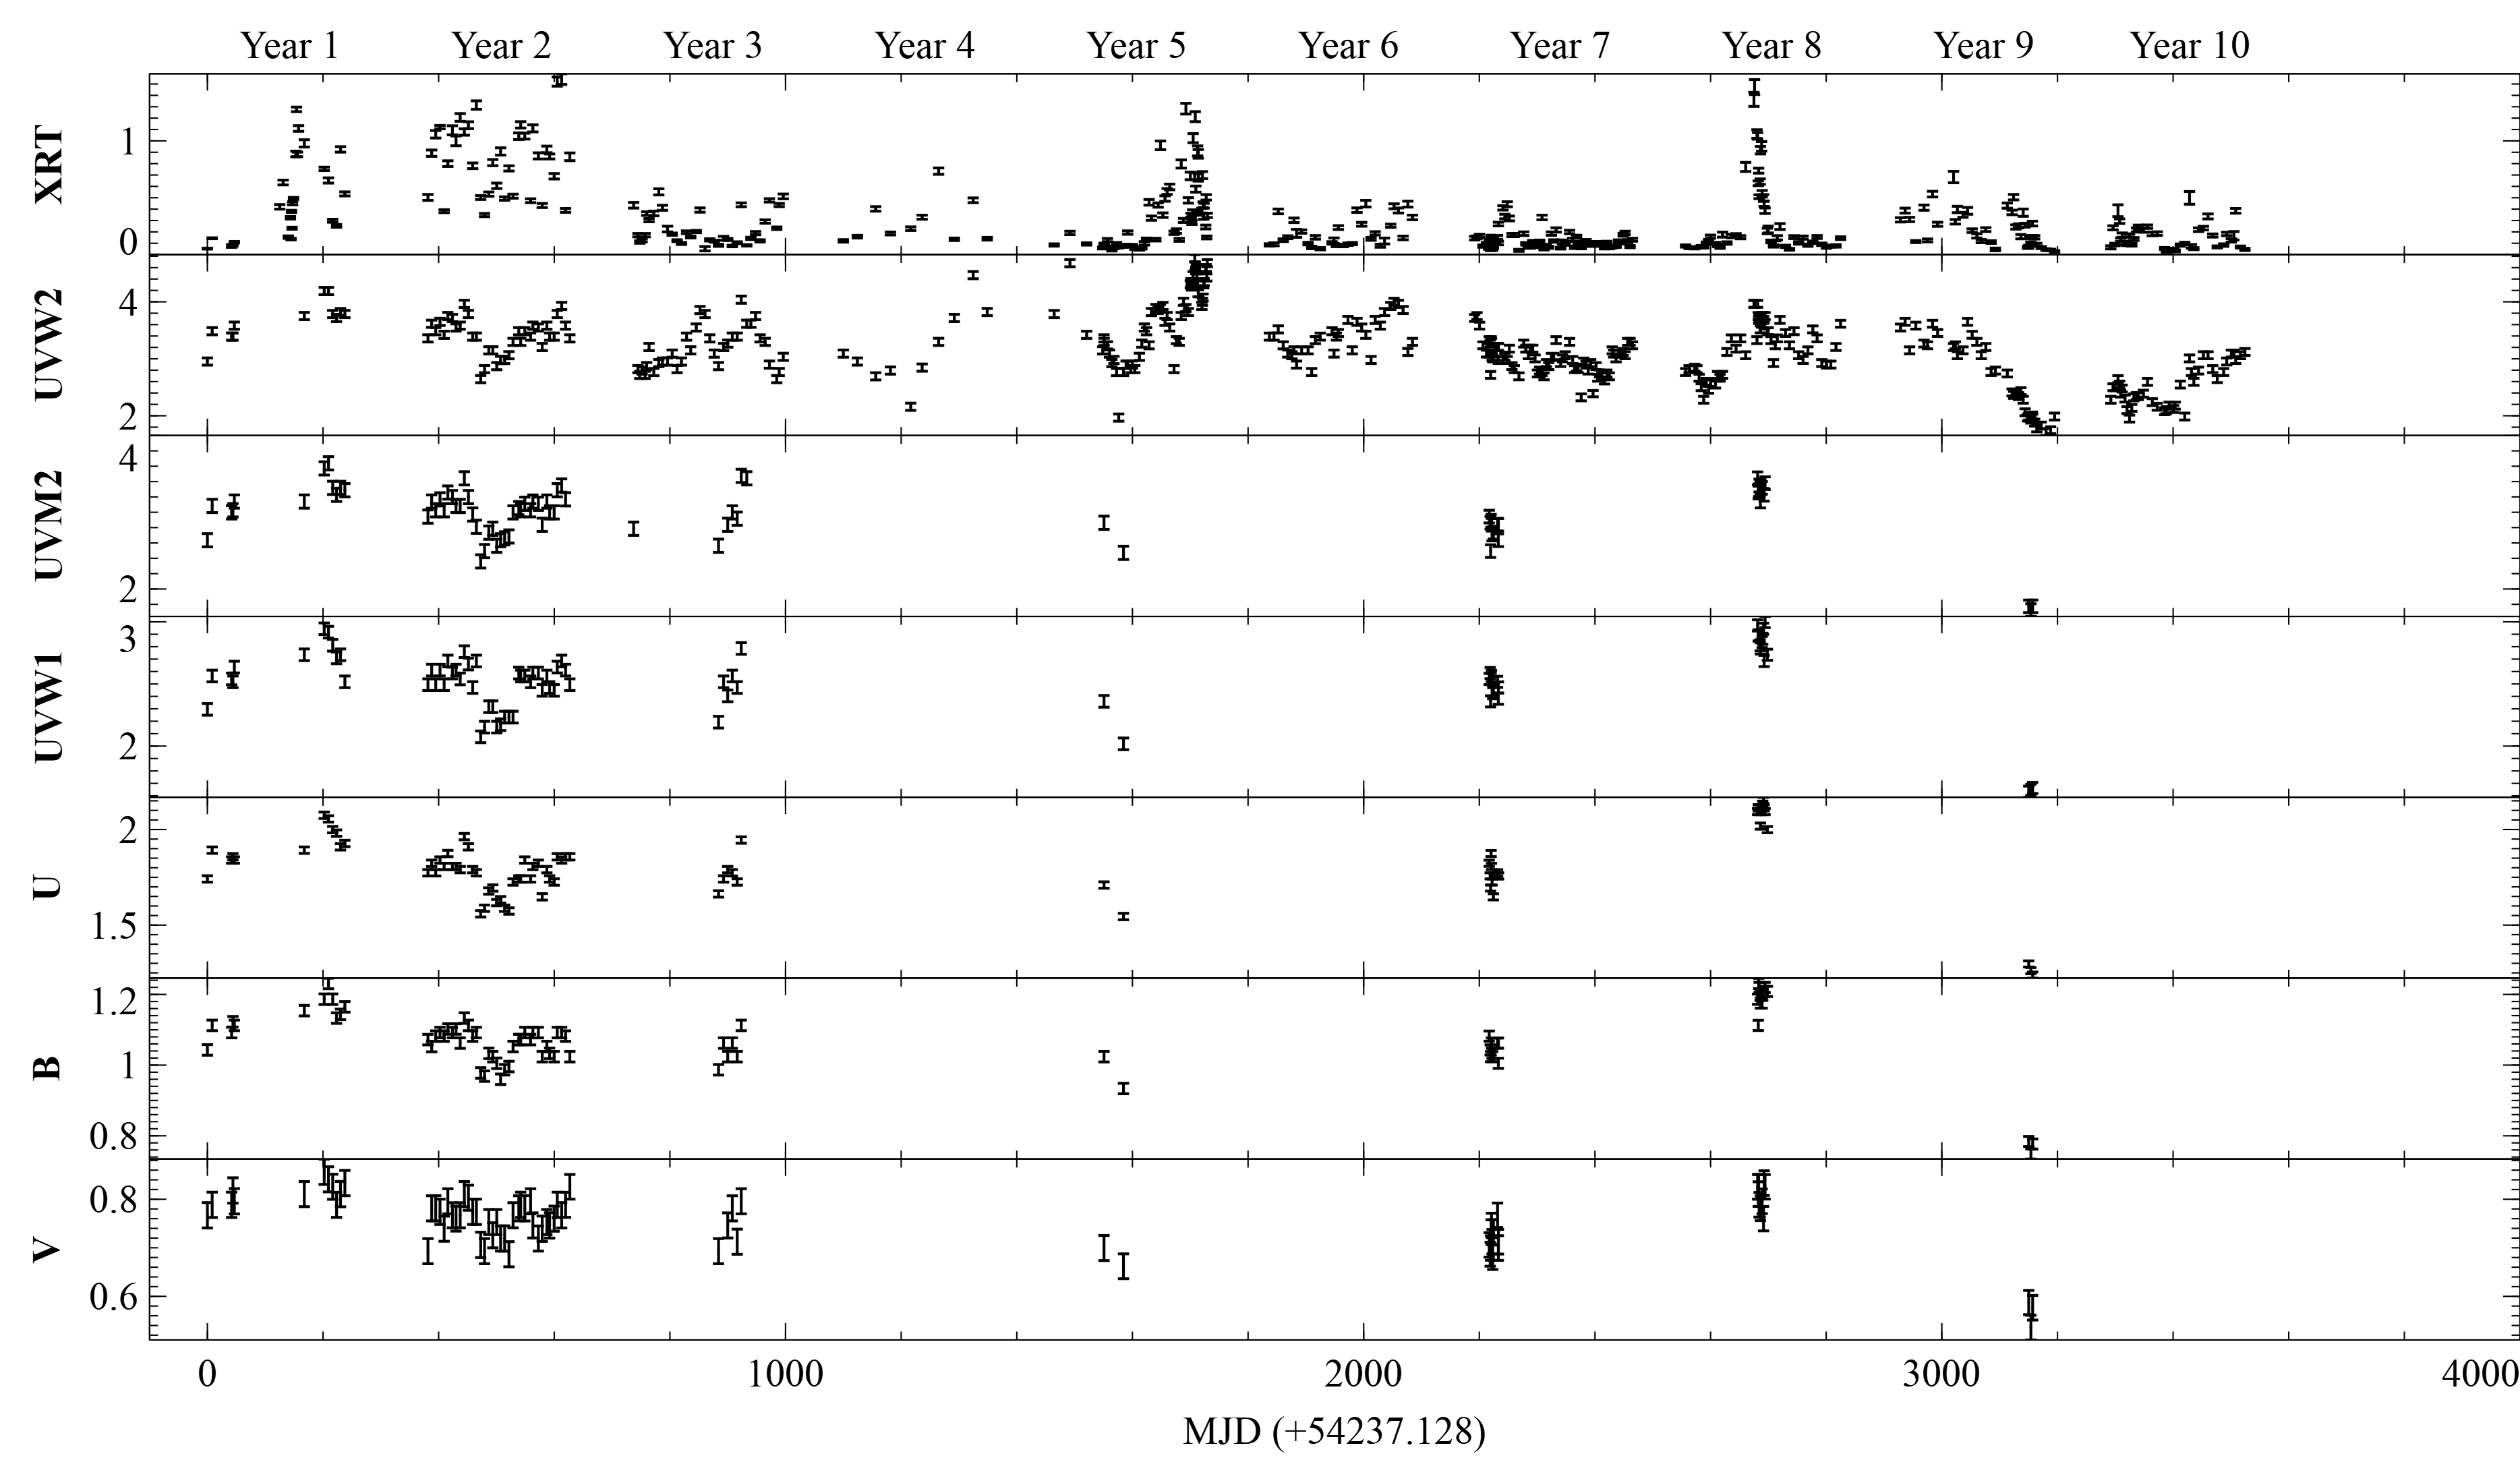
\includegraphics[width=0.8\linewidth]{mkn335Lightcurves}
	\caption{The \textit{Swift} XRT and UVOT light curves for \textbf{Mrk} 335 from 17 May 2007 to 31 Dec 2017. The XRT light curve is in counts s$^{-1}$. UVOT light curves are in units of $10^{-14}$erg s$^{-1}$cm$^{-2}$\AA$^{-1}$}
	\label{fig:mkn335LC}
\end{figure}

An overview of the data. This section will contain many figures.

\chapter{\sc Programming SFA} \label{programmingSFA}

\section{\sc SFA usage and description} \label{usageDescription}

A description of what SFA was developed for and its usage.

\section{\sc The SFA algorithm} \label{algorithm}

\subsection{\sc Process}

The logical process SFA follows to generate the structure function

\subsection{\sc Cost and Complexity} \label{costComplexity}

An overview of the general running cost and Big-Oh order of SFA

\section{\sc Expected Output} \label{expectedOutput}

What one should expect for results from running SFA

\chapter{\sc Results and Conclusions} \label{resultsConclusions}

\section{\sc Results} \label{results}

A review of the results of running SFA on observational data

\section{\sc Conclusions} \label{conclusions}

Theoretical conclusions based on the findings of SFA

\chapter{\sc Future Work} \label{futureWork}

Potential future work and applications of SFA


\appendix

\chapter{Structure Function} \label{appendixSFA}
\label{app:sfa}
If you wanted an appendix, it would go in like this.  It would be 
referenced using Appendix~\ref{app:sfa}.


\begin{singlespace}
\bibliography{SMU-HonorsThesis-template}
\end{singlespace}
\end{document}
